
%(BEGIN_QUESTION)
% Copyright 2011, Tony R. Kuphaldt, released under the Creative Commons Attribution License (v 1.0)
% This means you may do almost anything with this work of mine, so long as you give me proper credit

A {\it current transformer} is a donut-shaped device used to measure the amount of AC current through a conductor, providing isolation between the power conductor and the instrument circuit.  Their purpose is to serve as a permanent ``clamp-on'' ammeter for a high-current AC power conductor.  The power conductor passes through the center of the ``donut'' while a stepped-down current is generated in the secondary winding to pass through an AC ammeter:

$$\includegraphics[width=15.5cm]{i04760x01.eps}$$

Calculate the amount of current through the ammeter in this example circuit, given the line current and ratio shown.

\vskip 50pt

Next, calculate the amount of current registered by the same ratio CT for all three line conductors of a three-phase power system as shown here (still assuming 350 amps AC in each line), explaining your answer:

$$\includegraphics[width=15.5cm]{i04760x02.eps}$$

\vfil 

\underbar{file i04760}
\eject
%(END_QUESTION)





%(BEGIN_ANSWER)

This is a graded question -- no answers or hints given!

%(END_ANSWER)





%(BEGIN_NOTES)

In the single-conductor example, the CT acts to step line current down by a ratio of 600 to 5 (120 to 1).  Thus, a line current of 350 amps develops a CT secondary current of 2.9167 amps.

\vskip 10pt

When all three lines of a three-phase load are passed through the center of the CT, the CT ``sees'' the superposition of all three magnetic fields resulting from all three line currents.  Assuming no ground fault in the three-phase load, each and every amp flowing from the source to the load must be matched by an amp of current flowing from the load back to the source (i.e. a complete circuit).  This means the superposition of these three currents' magnetic fields must be zero, and therefore the CT will output 0 amps regardless of line current.

This phenomenon is perhaps most evident if we consider a Wye-connected load:

$$\includegraphics[width=15.5cm]{i04760x03.eps}$$

Kirchhoff's Current Law declares that the algebraic sum of all electric currents entering and exiting a node (such as the center of a Wye network) must be equal to zero.  Thus, the algebraic sum of all line currents in this Wye-connected load must be equal to zero, and therefore their magnetic fields must mutually cancel in the iron core of a toroid surrounding all three conductors.

\vskip 10pt

This sort of CT usage -- sometimes referred to as a {\it zero-sequence} CT -- is used to detect ground faults in a three-phase load.  Only if the load suffers a ground fault, where some current flows through an earth ground connection and does not return to the source through the three power lines passing through the CT's center, will the CT register any current at all.


%INDEX% Electronics review: 3-phase electrical power 
%INDEX% Electronics review: current transformer (CT)

%(END_NOTES)


